\documentclass[aps,prx,reprint,superscriptaddress,nofootinbib,floatfix]{revtex4-2}
\usepackage[utf8]{inputenc}
\usepackage[T1]{fontenc}
\usepackage{amsmath,amssymb,amsthm}
\usepackage{graphicx}
\usepackage{microtype}
\usepackage{xcolor}
\usepackage[colorlinks=true,linkcolor=blue!65!black,citecolor=blue!65!black,urlcolor=blue!65!black]{hyperref}

\newtheorem{proposition}{Proposition}

\begin{document}

\title{Finite-Size Thermal Protection in Compact Recursively Welded Codes}

\author{Harshil Avlani}
\affiliation{Department of Physics and Department of Electrical Engineering and Computer Science, Massachusetts Institute of Technology, Cambridge, Massachusetts 02139, USA}
\author{Rohan Bodke}
\affiliation{Department of Physics and Department of Electrical Engineering and Computer Science, Massachusetts Institute of Technology, Cambridge, Massachusetts 02139, USA}
\author{Rushil Shah}
\affiliation{Department of Physics and Department of Electrical Engineering and Computer Science, Massachusetts Institute of Technology, Cambridge, Massachusetts 02139, USA}
\author{Yichen Li}
\affiliation{Department of Physics and Department of Electrical Engineering and Computer Science, Massachusetts Institute of Technology, Cambridge, Massachusetts 02139, USA}

\date{November 2026 --- MIT 6.S980: Quantum Error Correction}

\begin{abstract}
The recursive welding architecture of Balasubramanian, Davydova, and Lin (BDL) motivates asking what finite-size thermal protection survives when recursive sheet-and-bridge codes are simplified to compact, explicit cells, and which retained features account for that protection. Adapting BDL's explicit refinement-and-doubling scheme, we construct a bounded-degree Calderbank--Shor--Steane (CSS) family that retains sheet duplication, bridge checks, and alternating protection of both Pauli sectors while reducing each step to a $2 \times 2$ cell with a single four-arm bridge cross. Locally, an auxiliary repetition-block model satisfies a per-wall minority bound $W_{\mathrm{wall}} \le 2V$ and a separate wall-majority quotient bound $C \le \frac{2}{5}V$ modulo four-wall coarse inversion, realized physically up to a generator factor of $11/5$. Under continuous-time single-qubit heat-bath dynamics with unit defect energy, completing a second alternating cycle at a $146.7\times$ qubit increase multiplies checkpointed joint quantum lifetime at $\beta = 6.5$ by $55.9 \pm 10.4$ on planar instances ($323 \to 47{,}387$ qubits) and by $4.38 \pm 0.97$ on rotated tori ($646 \to 94{,}774$ qubits). Torus cycles exhibit a warm-to-cold crossover near $\beta \approx 6.1$, whereas an added planar half-cycle ($423{,}559$ qubits) is bottlenecked by its un-welded $Z$ sector and gives no resolved gain ($1.18 \pm 0.28$). Weakening selected check couplings at fixed code space shows that coarse Cycle-$1$ welds affect cold lifetimes more strongly per check than equal-count, weight-matched fine Cycle-$2$ welds, though weakening either scale erases the two-cycle gain. Finally, we validate hierarchical readout and cadence sensitivity and delimit spatial implementation costs from three-dimensional ball packing, surface-collar expansion, and CSS check-leg wires.
\end{abstract}

\maketitle

\section{Motivation and Model}

Active quantum error correction protects stored states through repeated syndrome extraction, classical decoding, and recovery operations \cite{bravyi_bb2024}. Passive quantum memories pursue a different operational regime: stabilizer checks enter directly as local terms of a static Hamiltonian coupled to a cold bath at inverse temperature $\beta = 1/T$, so energetically costly defects tend to recombine during storage and classical decoding is performed only at readout \cite{quantumMemories, selfcorrecting4D, alicki4D}.

Raising the static energy barrier between logical sectors is necessary but not sufficient for passive protection, because thermal memory depends on the free-energy competition between defect energy penalties and configurational entropy \cite{chesi2010, siva2017, bergamaschi2025mixing}. Geometrically local two-dimensional stabilizer codes have constant energy barriers because isolated point defects move across sheets at zero energy cost \cite{selfcorrecting2D}, whereas non-planar or expander codes alter graph connectivity \cite{bravyi_bb2024, hong2025trivial, guo2026neutral}. In three dimensions, Michnicki's welded solid code achieved a power-law static energy barrier \cite{michnicki2014}, yet subsequent analysis showed that entropic proliferation of excitations limits its memory time to a finite temperature-dependent scale \cite{siva2017}. Haah's Cubic Code eliminates string logical operators and creates logarithmic energy barriers that yield steep low-temperature transients at small sizes \cite{haah2011cubic, yoshida2011, bravyi_haah2013}, though rapid thermalization has recently been proved at every positive temperature in its specified Davies bath setting \cite{stengele2026haah}. Three-dimensional topological and random layer codes establish rigorous regimes of partial self-correction with characteristic finite-size lifetime peaks \cite{layercodesydney, layercodesyale, williamson2026layer}.

Balasubramanian, Davydova, and Lin (BDL) \cite{selfcorrecting3D} recently proved that a three-dimensional passive self-correcting quantum memory exists by organizing welds recursively across scales. BDL present two related versions of their architecture: a randomized embedding proof whose asymptotic analysis invokes a spatial scale-dilation parameter near $5.4 \times 10^{24}$ per recursion step, and an explicit geometric refinement-and-doubling scheme (BDL Sec.~6.2) that routes duplicated sheets and two-rib bridges on a scale-$\ell = 8$ cubic grid ($56{,}312$ qubits in a single planar cycle) while deferring a complete thermal proof. In companion work on a modified welded family, Hayden Part~I \cite{hayden2026} establishes unperturbed quantum thermal memory stability together with zero-temperature perturbative stability against weak quantum perturbations, likewise employing large discretization cardinalities while deferring positive-temperature perturbed interior dynamics.

\begin{figure*}[t!]
  \centering
  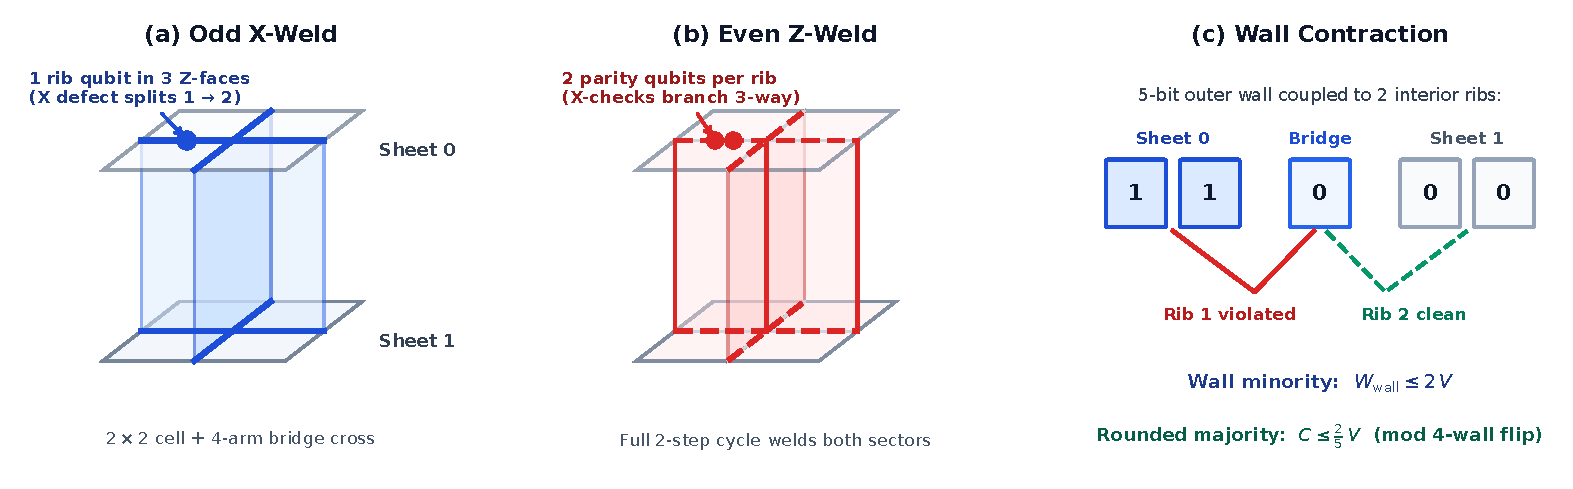
\includegraphics[width=0.98\textwidth]{../figures/fig_v19_1_construction.pdf}
  \caption{\textbf{BDL Correspondence, Compact Cell, and Local Bounds.} \textbf{(a)}~Adapting BDL Sec.~6.2, an odd step subdivides each face into $2 \times 2$, duplicates the sheet, and attaches a single-rib bridge cross where one physical rib qubit participates in three $Z$-face checks, splitting crossing $X$ defects from one into two. \textbf{(b)}~An even step places two parity qubits along each three-sheet rib so $X$-checks branch across sheets; holding seed and commutation rules fixed, pruning one bridge arm or merging $X$ and $Z$ welds into one step introduces weight-one $Z$ logicals and lowers dressed distance. \textbf{(c)}~On an auxiliary $2 \times 2$ cell, each five-bit outer wall satisfies $W_{\mathrm{wall}} \le 2V$ (Proposition~\ref{prop:wall}) and five-bit wall majority satisfies $C \le \frac{2}{5}V$ modulo simultaneous four-wall inversion (Proposition~\ref{prop:majority}).}
  \label{fig:construction}
\end{figure*}

Existence proofs at very large scale parameters leave a concrete finite-size question open: when BDL's Section~6.2 sheet-and-bridge hierarchy is stripped down to small, explicit recursive cells on bounded-degree graphs, what measurable thermal protection survives across accessible system sizes, and which architectural ingredients control it? Here \emph{compact} refers to a minimal recursive cell generating tractable finite-size instances for exact algebraic and numerical study, rather than an immediate hardware blueprint at hundreds of thousands of qubits.

To evaluate finite-size protection on a uniform footing, we study CSS Hamiltonians with unit check energy ($J = 1$),
\begin{equation}
  H \;=\; \frac{1}{2} \sum_{a} \bigl(I - S_a^X\bigr) \;+\; \frac{1}{2} \sum_{b} \bigl(I - S_b^Z\bigr),
  \label{eq:hamiltonian}
\end{equation}
so every violated stabilizer check adds $+1$ to the energy. Modeling weak contact with an uncorrelated single-qubit bath \cite{davies1974}, $X$ and $Z$ errors evolve from the clean ground state $e(0) = 0$ as independent continuous-time Markov chains in which flipping a qubit with energy change $\Delta E$ occurs at the heat-bath rate
\begin{equation}
  r(\Delta E) \;=\; \frac{1}{1 + e^{\beta \Delta E}}.
  \label{eq:glauber}
\end{equation}
Trajectories are generated without time-step discretization via the rejection-free Bortz--Kalos--Lebowitz (BKL) algorithm \cite{bkl1975}. Because exact bath sampling is distinct from continuous failure monitoring, we define our primary observable explicitly as the \emph{checkpointed first-detected failure time} $T_P$ ($P \in \{X, Z\}$) under readout after every flip for the first $16$ flips and at multiplicative intervals $t_{k+1} = (1 + \eta)\,t_k$ with baseline $\eta = 0.20$ thereafter (auditing $\eta \in [0, 0.50]$ in Sec.~\ref{sec:readout}). Under independent $X$ and $Z$ chains, joint quantum survival is $S_Q(t) = S_X(t)\,S_Z(t)$ with mean lifetime
\begin{equation}
  \tau_Q \;=\; \int_0^\infty S_X(t)\,S_Z(t)\,dt,
  \label{eq:tauq}
\end{equation}
estimated across all $n_X n_Z$ cross-sector trajectory pairs $\min(T_{X,i}, T_{Z,j})$ with standard errors obtained by bootstrapping independent trajectories within each sector ($2{,}000$ resamples). Whenever a non-limiting sector has right-censored runs at flip cap $C_P$ while the limiting sector is uncensored, $\min(C_X, T_Z) \le \min(T_X, T_Z) \le T_Z$ yields an exact full-cohort censoring bracket $[\tau_Q^{\mathrm{lo}}, \tau_Q^{\mathrm{hi}}]$.

\section{Compact Welded Family}
\label{sec:family}

On a single surface-code sheet, qubits sit on edges, face $Z$-checks detect $X$ errors, and vertex $X$-checks detect $Z$ errors. Once a pair of point defects is thermally created, flipping intervening edges moves them across the sheet at $\Delta E = 0$. BDL's Section~6.2 construction obstructs that free motion by welding duplicated sheets along interior bridges so a defect crossing a seam must violate an extra check on the adjoining sheet, alternating odd and even steps to protect both Pauli sectors.

\begin{table}[b!]
\caption{\textbf{Compact Code Family Specifications.} Boundary family, recursion step $s$ (completed cycles $C_r$ at $s = 2r$), physical qubits $N$, encoded qubits $K = N - \operatorname{rank} H_X - \operatorname{rank} H_Z$, exact sector distances $(d_X, d_Z)$ where enumerated or pushed logical upper weights $\le (w_{\bar{X}}, w_{\bar{Z}})$, maximum check weights $(w_X, w_Z)$, and maximum total check degree per qubit $\deg_{\max}$.}
\label{tab:codes}
{\scriptsize
\setlength{\tabcolsep}{1.8pt}
\begin{ruledtabular}
\begin{tabular}{llccccc}
Instance & Step & $N$ & $K$ & $(d_X, d_Z)$ / Up. & $(w_X, w_Z)$ & $\deg$ \\
\colrule
Planar $2{\times}2$ & $s{=}0$ ($C_0$) & $2$ & $1$ & $(2, 1)$ & $(0, 2)$ & $1$ \\
Planar $2{\times}2$ & $s{=}1$ (half) & $19$ & $1$ & $(6, 2)$ & $(5, 4)$ & $6$ \\
Planar $2{\times}2$ & $s{=}2$ ($C_1$) & $323$ & $1$ & ${\le}(11, 10)$ & $(6, 6)$ & $7$ \\
Planar $2{\times}2$ & $s{=}3$ (half) & $2{,}911$ & $1$ & ${\le}(42, 20)$ & $(7, 6)$ & $7$ \\
Planar $2{\times}2$ & $s{=}4$ ($C_2$) & $47{,}387$ & $1$ & ${\le}(92, 100)$ & $(7, 7)$ & $7$ \\
Planar $2{\times}2$ & $s{=}5$ (half) & $423{,}559$ & $1$ & --- & $(7, 6)$ & $7$ \\
\colrule
Torus $2{\times}2$ & $s{=}0$ ($C_0$) & $4$ & $2$ & $(2, 2)$ & $(4, 4)$ & $4$ \\
Torus $2{\times}2$ & $s{=}1$ (half) & $38$ & $2$ & $({\le}8, 4)$ & $(5, 4)$ & $6$ \\
Torus $2{\times}2$ & $s{=}2$ ($C_1$) & $646$ & $2$ & ${\le}(18, 20)$ & $(6, 6)$ & $7$ \\
Torus $2{\times}2$ & $s{=}3$ (half) & $5{,}822$ & $2$ & ${\le}(76, 40)$ & $(7, 6)$ & $7$ \\
Torus $2{\times}2$ & $s{=}4$ ($C_2$) & $94{,}774$ & $2$ & ${\le}(176, 200)$ & $(7, 7)$ & $7$ \\
\colrule
Planar $3{\times}3$ & $s{=}1$ (half) & $41$ & $1$ & $({\le}8, 3)$ & $(5, 4)$ & $6$ \\
Planar $3{\times}3$ & $s{=}2$ ($C_1$) & $1{,}271$ & $1$ & ${\le}(22, 21)$ & $(6, 6)$ & $7$ \\
Planar $3{\times}3$ & $s{=}3$ (half) & $24{,}449$ & $1$ & ${\le}(128, 63)$ & $(7, 6)$ & $7$ \\
\colrule
2-Rib Direct & $s{=}2$ ($C_1$) & $1{,}480$ & $1$ & ${\le}(20, 24)$ & $(5, 6)$ & $6$ \\
$\ell{=}8$ Grid & $s{=}2$ ($C_1$) & $56{,}312$ & $1$ & ${\le}(144, 144)$ & $(6, 6)$ & $7$ \\
\end{tabular}
\end{ruledtabular}
}
\end{table}

Our compact family adapts BDL Section~6.2 with four explicit simplifications (Fig.~\ref{fig:construction}a and Table~\ref{tab:codes}). We retain edge subdivision, two-sheet duplication, and alternating $X$- and $Z$-weld bridges. First, we reduce the subdivision factor from $\ell = 8$ to $L = 2$ (and $L = 3$ in Sec.~\ref{sec:readout}). Second, we replace BDL's two parallel interior ribs per cell (used in BDL Sec.~6.2.6 to keep interior cleanup pockets disjoint) with a single central four-arm cross. Third, we study both an open planar seed $[[2, 1, (2, 1)]]$ ($N = 2, K = 1$, sector distances $(d_X, d_Z) = (2, 1)$ so CSS distance $d = \min(d_X, d_Z) = 1$) and a boundaryless rotated torus seed $[[4, 2, 2]]$ ($N = 4, K = 2$, $(d_X, d_Z) = (2, 2)$). Fourth, we evaluate the resulting bounded-degree interaction graph directly ($\deg_{\max} \le 7$, check weights $\le 7$), separating graph-level thermal dynamics from three-dimensional Euclidean routing.

Explicit CSS parity-check matrices $(H_X, H_Z)$ are generated at every step by a deterministic cellular sheaf rule (Appendix~\ref{app:css}). On an ordinary interior edge ($d = 2$ incident faces) or an odd-step $X$-weld seam ($d \ge 3$), one physical qubit participates in all $d$ incident face $Z$-checks (Fig.~\ref{fig:construction}a). On an even-step $Z$-weld seam with ordered incident faces $f_0, \dots, f_{d-1}$, $d - 1$ physical qubits couple adjacent face pairs $\{f_j, f_{j+1}\}$ in $H_Z$ while vertex $X$-checks span the minimal-weight local kernel of the incident edge constraints, ensuring $H_X H_Z^T = 0 \pmod 2$ and preserving $K = N - \operatorname{rank} H_X - \operatorname{rank} H_Z$ across all recursion steps (Fig.~\ref{fig:construction}b). Because odd steps add $X$-welds while subdividing $Z$-distances only linearly on sheets, a \emph{complete two-step cycle} ($s = 2r$) is the natural unit of two-sector quantum protection.

Holding the seed and local sheaf commutation rules fixed, two further simplifications degrade logical protection (Fig.~\ref{fig:construction}b). Pruning one arm of the bridge cross to form a three-arm T-bridge opens an interior seam boundary that increases torus $K$ from $2$ to $1{,}004$ by step~$4$ and introduces eight weight-one $Z$ logical operators on planar Cycle~$1$ (lowering dressed seed-logical distance to $(6, 5)$). Merging horizontal $X$-welds and vertical $Z$-welds into a single doubling step creates a four-sheet corner clash at the cross center that leaves dressed distance $d_Z = 1$. These are construction-specific ablations under fixed local rules rather than a universal minimality proof over all possible gadgets.

To examine local defect confinement within one $2 \times 2$ even-weld cell, label the four cyclic subfaces of Sheet~$0$, Sheet~$1$, and the bridge cross by $a_i, b_i, c_i \in \{0, 1\}$ ($i \in \mathbb{Z}_4$; Fig.~\ref{fig:construction}c). Let $\chi$ equal $1$ when a tuple is not monochromatic and $0$ otherwise. The nine interior repetition blocks count
\begin{equation}
\begin{aligned}
  V \;=\;& \sum_{i=0}^3 \chi(a_i, a_{i+1}, c_i) + \sum_{i=0}^3 \chi(b_i, b_{i+1}, c_i) \\
         &+ \chi(c_0, c_1, c_2, c_3).
\end{aligned}
  \label{eq:vrep}
\end{equation}
Outer wall $i$ carries five boundary bits with sum $n_i = a_i + a_{i+1} + b_i + b_{i+1} + c_i$ and per-wall minority weight
\begin{equation}
  W_{\mathrm{wall}} \;=\; \sum_{i=0}^3 \min(n_i, 5 - n_i).
  \label{eq:wwall}
\end{equation}

\begin{proposition}[Wall-Minority Bound]
\label{prop:wall}
Every nonconstant labeling of the $2 \times 2$ auxiliary cell satisfies $V \ge 2$ and $W_{\mathrm{wall}} \le 2V$, achieved with equality only on the four full-sheet patterns ($W_{\mathrm{wall}} = 8, V = 4$).
\end{proposition}

\begin{proof}
For wall $i$, if both $\chi(a_i, a_{i+1}, c_i)$ and $\chi(b_i, b_{i+1}, c_i)$ vanish, all five wall bits equal $c_i$ and $\min(n_i, 5 - n_i) = 0$. Otherwise at least one of the two triples is violated and $\min(n_i, 5 - n_i) \le 2$, so $\min(n_i, 5 - n_i) \le 2\bigl[\chi(a_i, a_{i+1}, c_i) + \chi(b_i, b_{i+1}, c_i)\bigr]$. Summing over $i \in \mathbb{Z}_4$ gives $W_{\mathrm{wall}} \le 2V$.
\end{proof}

Hierarchical coarse-graining uses the rounded wall majority $q_i = \mathbf{1}[n_i \ge 3]$ modulo simultaneous four-wall inversion, $C = \min\bigl(\sum_i q_i,\, 4 - \sum_i q_i\bigr)$. Because patterns such as $a = 0000, b = 0111, c = 0110$ give $(W_{\mathrm{wall}}, V, C) = (6, 5, 2)$ with $C > W_{\mathrm{wall}}/5$, the rounded bound requires a separate argument (proved in Appendix~\ref{app:css}).

\begin{proposition}[Wall-Majority Quotient Bound]
\label{prop:majority}
Every labeling of the $2 \times 2$ auxiliary cell satisfies $C \le \frac{2}{5}V$ (attained on $92$ of $4{,}096$ states). On the $24$-variable, $27$-hyperedge $3 \times 3$ single-cross auxiliary cell, $W_{\mathrm{wall}} \le 2V$ and $C \le \frac{2}{7}V$ hold across all $2^{24}$ labelings.
\end{proposition}

In the physical CSS coboundary $H_Z^T m$ on dual face subsets $m \in \mathbb{F}_2^F$, the $19$ interior parity qubits of a $2 \times 2$ cell satisfy $V(m) \le V_{\mathrm{phys}}(m) \le \frac{11}{5}V(m)$, $W_{\mathrm{wall}}(m) \le V_{\mathrm{phys}}(m)$, and $C(m) \le \frac{2}{5}V_{\mathrm{phys}}(m)$, while toggling a coarse parent face $y_P \in \{0, 1\}$ lifts to simultaneous inversion across all four walls of cell $P$ (Appendix~\ref{app:css}). Across multiple cells on a $3 \times 3$ periodic seed torus ($V_0 = 9, E_0 = 18, F_0 = 9$), however, BDL's two-rib $X$-weld creates $\dim\ker H_Z^T = 37$ independent closed syndrome pockets ($V_0 + E_0 + F_0 + 1$ plus $9$ split-bridge cycles), whereas our one-rib cell merges adjacent pockets across the shared rib down to $\dim\ker H_Z^T = 10 = V_0 + 1$. While failure of BDL's three-stage pocket partition does not rule out all alternative multi-cell cleanup arguments, a global thermal theorem for one-rib cells remains open.

\section{Complete-Cycle Protection}
\label{sec:lifetimes}

\begin{figure*}[t!]
  \centering
  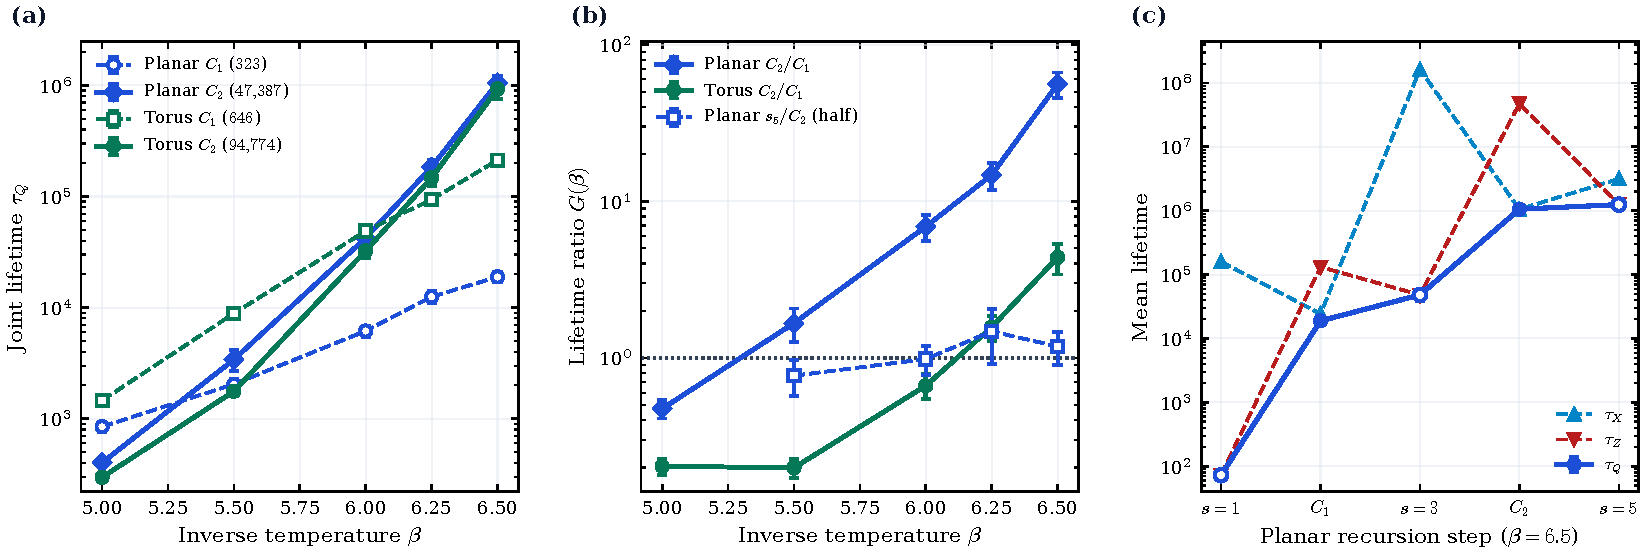
\includegraphics[width=0.98\textwidth]{../figures/fig_v19_2_lifetimes.pdf}
  \caption{\textbf{Complete-Cycle Lifetime Gains, Torus Crossover, and Sector Bottlenecks.} \textbf{(a)}~Checkpointed joint lifetime $\tau_Q$ ($\pm 1\,\mathrm{SEM}$) versus physical qubit count $N$ at fixed $\beta \in \{5.5, 6.0, 6.5\}$ for planar (blue) and torus (green) families; filled markers connected by solid lines denote completed cycles ($s = 2, 4$), and open markers denote planar half-cycles ($s = 1, 3, 5$). \textbf{(b)}~Complete-cycle gain $G_1(\beta) = \tau_Q(C_2, \beta)/\tau_Q(C_1, \beta)$ ($\pm 1\,\mathrm{SE}$, each at $146.7\times$ qubit growth) alongside the planar half-step ratio $\tau_Q(s_5)/\tau_Q(C_2)$ ($8.9\times$ qubits), showing the torus warm-to-cold crossover near $\beta \approx 6.1$. \textbf{(c)}~Sector-resolved planar lifetimes $(\tau_X, \tau_Z, \tau_Q)$ at $\beta = 6.5$, illustrating how alternating steps trade the limiting Pauli sector.}
  \label{fig:lifetimes}
\end{figure*}

\begin{table*}[t!]
\caption{\textbf{Thermal Lifetimes, Sector Breakdown, and Complete-Cycle Gains ($J = 1, \eta = 0.20$).} Inverse temperature $\beta$, sector means $\tau_X, \tau_Z$ with $[c_P / n_P]$ denoting right-censored runs over total independent trajectories, joint lifetime $\tau_Q \pm \mathrm{SEM}$ (with exact full-cohort censoring bracket gap $\Delta_{\mathrm{cens}}$; $0.0\%$ whenever every limiting-sector run fails below the non-limiting flip cap), complete-cycle or half-step gain $G(\beta) \pm \mathrm{SE}$, and activation slope $\hat{\Delta}_{\mathrm{eff}} \pm \mathrm{SE}$ over the stated $\beta$ window.}
\label{tab:lifetimes}
{\scriptsize
\setlength{\tabcolsep}{2.2pt}
\begin{ruledtabular}
\begin{tabular}{llcccccl}
Instance ($N, K$) & $\beta$ & $\tau_X$ $[c_X/n_X]$ & $\tau_Z$ $[c_Z/n_Z]$ & $\tau_Q \pm \mathrm{SEM}$ ($\Delta_{\mathrm{cens}}$) & Gain $G(\beta)$ & $\hat{\Delta}_{\mathrm{eff}}$ [$\beta$] \\
\colrule
Planar $C_1$ ($323, 1$) & $5.50$ & $(2.68{\pm}0.28){\times}10^3$ $[0/96]$ & $(1.25{\pm}0.13){\times}10^4$ $[0/96]$ & $(2.04{\pm}0.22){\times}10^3$ ($0\%$) & --- & $2.12{\pm}0.09$ $[5.0,6.5]$ \\
Planar $C_1$ ($323, 1$) & $6.50$ & $(2.42{\pm}0.27){\times}10^4$ $[0/96]$ & $(1.32{\pm}0.15){\times}10^5$ $[0/96]$ & $(1.89{\pm}0.20){\times}10^4$ ($0\%$) & --- & \\
Planar $C_2$ ($47{,}387, 1$) & $5.50$ & $(3.40{\pm}0.72){\times}10^3$ $[0/36]$ & $>1.33{\times}10^7$ $[33/36]$ & $(3.40{\pm}0.71){\times}10^3$ ($0\%$) & $1.67{\pm}0.40$ ($C_1$) & $5.06{\pm}0.20$ $[5.0,6.5]$ \\
Planar $C_2$ ($47{,}387, 1$) & $6.00$ & $(4.24{\pm}0.65){\times}10^4$ $[0/36]$ & $>2.63{\times}10^7$ $[36/36]$ & $(4.24{\pm}0.64){\times}10^4$ ($0\%$) & $6.89{\pm}1.33$ ($C_1$) & \\
Planar $C_2$ ($47{,}387, 1$) & $6.50$ & $(1.06{\pm}0.15){\times}10^6$ $[0/36]$ & $>4.77{\times}10^7$ $[36/36]$ & $(1.06{\pm}0.15){\times}10^6$ ($0\%$) & $55.9{\pm}10.4$ ($C_1$) & \\
Planar $s_5$ ($423{,}559, 1$) & $6.50$ & $>3.15{\times}10^6$ $[12/12]$ & $(1.26{\pm}0.21){\times}10^6$ $[0/20]$ & $(1.25{\pm}0.21){\times}10^6$ ($1.2\%$) & $1.18{\pm}0.28$ ($C_2$) & $6.14{\pm}0.28$ $[5.5,6.5]$ \\
\colrule
Torus $C_1$ ($646, 2$) & $5.50$ & $(8.92{\pm}0.88){\times}10^3$ $[0/96]$ & $(1.15{\pm}0.12){\times}10^7$ $[0/96]$ & $(8.87{\pm}0.87){\times}10^3$ ($0\%$) & --- & $3.32{\pm}0.08$ $[5.0,6.5]$ \\
Torus $C_1$ ($646, 2$) & $6.00$ & $(4.89{\pm}0.51){\times}10^4$ $[0/96]$ & $(1.33{\pm}0.14){\times}10^8$ $[0/96]$ & $(4.89{\pm}0.51){\times}10^4$ ($0\%$) & --- & \\
Torus $C_1$ ($646, 2$) & $6.50$ & $(2.12{\pm}0.23){\times}10^5$ $[0/96]$ & $(1.95{\pm}0.21){\times}10^9$ $[0/96]$ & $(2.12{\pm}0.23){\times}10^5$ ($0\%$) & --- & \\
Torus $C_2$ ($94{,}774, 2$) & $5.50$ & $(1.76{\pm}0.16){\times}10^3$ $[0/36]$ & $>2.19{\times}10^7$ $[36/36]$ & $(1.76{\pm}0.16){\times}10^3$ ($0\%$) & $0.20{\pm}0.03$ ($C_1$) & $5.04{\pm}0.41$ $[5.0,6.5]$ \\
Torus $C_2$ ($94{,}774, 2$) & $6.00$ & $(3.25{\pm}0.48){\times}10^4$ $[0/36]$ & $>6.15{\times}10^7$ $[24/24]$ & $(3.25{\pm}0.48){\times}10^4$ ($0\%$) & $0.66{\pm}0.12$ ($C_1$) & \\
Torus $C_2$ ($94{,}774, 2$) & $6.25$ & $(1.47{\pm}0.23){\times}10^5$ $[0/36]$ & $>1.02{\times}10^8$ $[24/24]$ & $(1.47{\pm}0.22){\times}10^5$ ($0\%$) & $1.57{\pm}0.29$ ($C_1$) & \\
Torus $C_2$ ($94{,}774, 2$) & $6.50$ & $(9.30{\pm}1.81){\times}10^5$ $[0/36]$ & $>1.70{\times}10^8$ $[24/24]$ & $(9.30{\pm}1.76){\times}10^5$ ($0\%$) & $4.38{\pm}0.97$ ($C_1$) & \\
\colrule
$3{\times}3$ $C_1$ ($1{,}271, 1$) & $6.50$ & $(8.83{\pm}1.28){\times}10^3$ $[0/80]$ & $(1.76{\pm}0.20){\times}10^6$ $[0/80]$ & $(8.83{\pm}1.28){\times}10^3$ ($0\%$) & --- & $2.17{\pm}0.07$ $[5.0,7.5]$ \\
$3{\times}3$ $C_1$ ($1{,}271, 1$) & $7.50$ & $(7.45{\pm}0.89){\times}10^4$ $[0/80]$ & $(9.11{\pm}1.12){\times}10^7$ $[0/80]$ & $(7.45{\pm}0.89){\times}10^4$ ($0\%$) & --- & \\
$3{\times}3$ $s_3$ ($24{,}449, 1$) & $6.50$ & $>3.41{\times}10^7$ $[15/16]$ & $(3.86{\pm}0.61){\times}10^3$ $[0/32]$ & $(3.86{\pm}0.61){\times}10^3$ ($0\%$) & $0.44{\pm}0.10$ ($C_1$) & $2.83{\pm}0.16$ $[5.0,7.5]$ \\
$3{\times}3$ $s_3$ ($24{,}449, 1$) & $7.50$ & $>1.12{\times}10^8$ $[16/16]$ & $(1.69{\pm}0.32){\times}10^5$ $[0/32]$ & $(1.69{\pm}0.32){\times}10^5$ ($0\%$) & $2.27{\pm}0.51$ ($C_1$) & \\
\colrule
2-Rib Direct ($1{,}480, 1$) & $6.50$ & $(1.74{\pm}0.19){\times}10^5$ $[0/80]$ & $(1.54{\pm}0.18){\times}10^7$ $[0/80]$ & $(1.74{\pm}0.19){\times}10^5$ ($0\%$) & --- & $3.21{\pm}0.11$ $[5.0,6.5]$ \\
$\ell{=}8$ Grid ($56{,}312, 1$) & $6.50$ & $394{\pm}33$ $[0/28]$ & $>1.19{\times}10^6$ $[1/28]$ & $394{\pm}33$ ($0\%$) & $0.0023$ ($1{,}480$q) & $1.31{\pm}0.15$ $[5.0,7.0]$ \\
\end{tabular}
\end{ruledtabular}
}
\end{table*}

Figure~\ref{fig:lifetimes} and Table~\ref{tab:lifetimes} present our central empirical test: how joint and sector-resolved lifetimes evolve when another complete cycle of alternating welding is added, using global Union-Find cluster decoding with local $\mathbb{F}_2$ cluster solves \cite{delfosse_uf, delfosse_qldpc_uf, panteleev_bposd} at readout. Rather than comparing the largest code against a weak odd-step baseline, we evaluate the complete-cycle gain
\begin{equation}
  G_r(\beta) \;=\; \frac{\tau_Q(C_{r+1}, \beta)}{\tau_Q(C_r, \beta)},
  \label{eq:gain}
\end{equation}
alongside the accompanying physical qubit factor. Between Cycle~$1$ ($s = 2$) and Cycle~$2$ ($s = 4$), qubit counts grow by $146.7\times$ in both boundary families ($323 \to 47{,}387$ planar; $646 \to 94{,}774$ torus), providing one nontrivial completed-cycle increment per family.

Adding a complete cycle does not increase lifetime at every temperature; instead, both families exhibit an explicit warm-to-cold crossover (Fig.~\ref{fig:lifetimes}a,b). In the warm regime $\beta = 5.0$, adding $146.7\times$ more qubits multiplies the number of nucleation sites faster than weld barriers suppress escape, yielding $G_1(5.0) = 0.47 \pm 0.06$ on planar sheets and $G_1(5.0) = 0.20 \pm 0.02$ on tori. On planar instances, $G_1(\beta)$ crosses unity near $\beta \approx 5.3$ and rises sharply to $6.89 \pm 1.33$ at $\beta = 6.0$, $14.7 \pm 2.9$ at $\beta = 6.25$, and $55.9 \pm 10.4$ at $\beta = 6.5$ ($95\%$ CI $[38.2, 79.3]$). On boundaryless rotated tori---whose Cycle~$1$ baseline is already $11.2\times$ longer-lived than planar Cycle~$1$ at $\beta = 6.5$ because open boundary paths are absent---Cycle~$2$ remains shorter-lived across $\beta \in \{5.0, 5.5, 6.0\}$ ($G_1(6.0) = 0.66 \pm 0.12$), crosses Cycle~$1$ between $\beta = 6.0$ and $6.25$ ($G_1(6.25) = 1.57 \pm 0.29$, $95\%$ CI $[1.08, 2.23]$), and reaches $G_1(6.5) = 4.38 \pm 0.97$ ($95\%$ CI $[2.85, 6.59]$; rising further to $13.3$ at $\beta = 6.65$, where $\tau_X$ reaches $(5.26 \pm 0.82)\times 10^6$ vs.\ $(3.97 \pm 0.43)\times 10^5$ on Cycle~$1$). Because only two completed cycles are accessible, this crossover marks a finite-size operating boundary rather than a thermodynamic critical temperature.

Sector-resolved lifetimes $(\tau_X, \tau_Z)$ explain why half-cycles behave differently from completed cycles (Fig.~\ref{fig:lifetimes}c). Every odd step ($X$-weld) boosts $\tau_X$ by several orders of magnitude while subdividing sheets without adding a new $Z$-weld, shifting the bottleneck to $\tau_Z$; every even step ($Z$-weld) boosts $\tau_Z$ past $10^7$ and returns the bottleneck to $\tau_X$. On the final planar half-step $C_2 \to s_5$ ($47{,}387 \to 423{,}559$ qubits, an $8.94\times$ qubit increase), $\tau_X(6.5)$ exceeds $3.15 \times 10^6$ while $\tau_Z(6.5) = (1.26 \pm 0.21) \times 10^6$ limits $\tau_Q(6.5)$ to $(1.25 \pm 0.21) \times 10^6$ (exact full-cohort censoring bracket $[1.248, 1.262] \times 10^6$, a $+1.17\%$ deterministic span well inside the $\pm 17\%$ sampling error). The resulting half-step ratio $1.18 \pm 0.28$ ($95\%$ CI $[0.76, 1.82]$) is not statistically resolved above unity, confirming that joint memory gains require protecting both sectors over a full cycle.

Over $\beta \in [5.0, 6.5]$, weighted Arrhenius fits give empirical activation slopes $\hat{\Delta}_{\mathrm{eff}} = \partial_\beta \ln \tau_Q$ rising from $2.12 \pm 0.09$ to $5.06 \pm 0.20$ across planar cycles and from $3.32 \pm 0.08$ to $5.04 \pm 0.41$ across torus cycles (Table~\ref{tab:lifetimes}). Under the same bath convention on finite instances, our simulated 2D Toric and active-fault-tolerant Bivariate Bicycle codes exhibit flat activation slopes across size ($\hat{\Delta}_{\mathrm{eff}} \approx 1.8\text{--}3.2$), while simulated Cubic and random layer instances display turnover or slower growth over tested ranges. Because fitted slopes depend on Hamiltonian normalization, bath dynamics, readout, and temperature window, we treat $\hat{\Delta}_{\mathrm{eff}}$ strictly as an empirical summary of these finite-size simulations rather than a universal barrier ranking or proof of asymptotic self-correction.

\section{Scale-Selective Coupling Test}
\label{sec:intervention}

\begin{figure*}[t!]
  \centering
  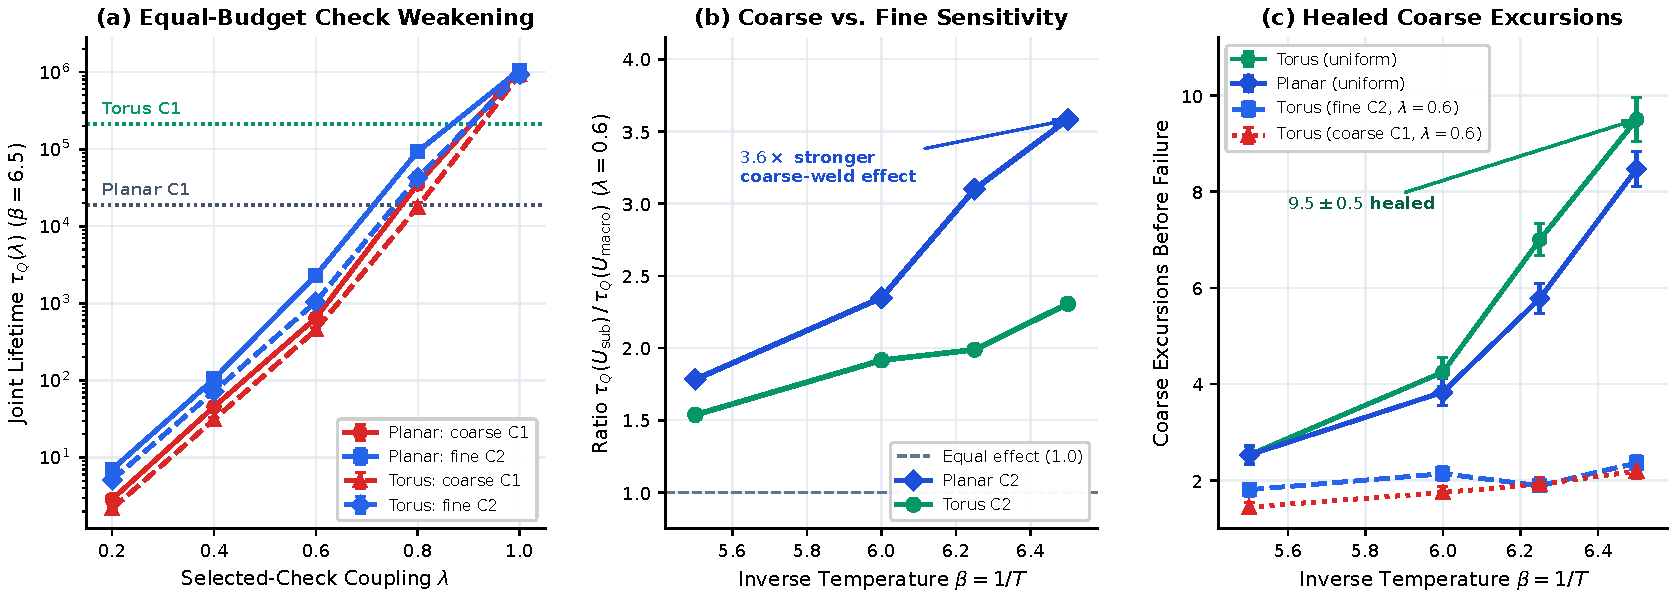
\includegraphics[width=0.98\textwidth]{../figures/fig_v19_3_intervention.pdf}
  \caption{\textbf{Scale-Selective Coupling Intervention and Coarse Excursions.} \textbf{(a)}~Joint lifetime $\tau_Q(\lambda)$ at $\beta = 6.5$ on fixed Cycle-$2$ planar ($47{,}387$q) and torus ($94{,}774$q) codes when weakening coarse Cycle-$1$ welds ($U_{\mathrm{macro}}$, red) versus an equal-count, exact-weight-matched subset of fine Cycle-$2$ sub-cell welds ($U_{\mathrm{sub}}$, blue); horizontal dotted lines mark Cycle-$1$ baselines. \textbf{(b)}~Sensitivity ratio $\tau(U_{\mathrm{sub}})/\tau(U_{\mathrm{macro}})$ across $\beta$, showing stronger sensitivity to coarse welds as temperature cools, especially in the $Z$ sector ($\lambda = 0.4$). \textbf{(c)}~Mean Cycle-$1$ coarse syndrome excursions per trajectory before failure, rising to $9.5 \pm 0.5$ on the uniform cold torus.}
  \label{fig:intervention}
\end{figure*}

Comparing $C_1$ and $C_2$ changes physical qubit count, code distance, and the number of Hamiltonian terms simultaneously. To test how multi-scale check organization contributes to lifetime on a \emph{fixed} code space, we assign every check of $C_2$ to its recursion step of origin and deform the Hamiltonian to
\begin{equation}
  H(\lambda; U) = \frac{1}{2} \sum_{a \notin U} (I - S_a) + \frac{\lambda}{2} \sum_{a \in U} (I - S_a), \quad 0 < \lambda \le 1.
  \label{eq:hlambda}
\end{equation}
Because $\lambda > 0$, the ground space, encoded dimension $K$, logical operators, check supports, and code distances remain unchanged; only the thermal energy barriers on $U$ are scaled by $\lambda$.

On both planar $C_2$ ($47{,}387$ qubits) and torus $C_2$ ($94{,}774$ qubits), we compare two disjoint check sets matched identically in check count, Pauli sector, and exact check-weight histogram: $U_{\mathrm{macro}}$ comprises coarse Cycle-$1$ bridge $Z$-checks and Cycle-$1$ seam $X$-checks ($5{,}034$ $Z$-checks and $6{,}176$ $X$-checks on planar; $10{,}008$ and $12{,}352$ on torus), while $U_{\mathrm{sub}}$ is a spatially strided subset of fine Cycle-$2$ sub-cell bridge $Z$-checks and Cycle-$2$-only seam $X$-checks with the identical weight breakdown (e.g., $1{,}920$ weight-$4$, $4{,}800$ weight-$5$, $3{,}240$ weight-$6$, and $48$ weight-$7$ $Z$-checks on the torus). What cannot be matched simultaneously at equal check count is fractional layer coverage: because $C_2$ contains roughly $2.3\times$ more fine bridges than coarse bridges, $U_{\mathrm{macro}}$ covers $98\text{--}99.7\%$ of Cycle-$1$ welds whereas $U_{\mathrm{sub}}$ covers $44\%$ of Cycle-$2$ $Z$-welds and $46\%$ of pure Cycle-$2$ $X$-welds. We therefore also evaluate $U_{\mathrm{C2,all}}$, which weakens $100\%$ of Cycle-$2$ welds ($23{,}040$ $Z$-checks and $43{,}752$ $X$-checks on the torus).

Figure~\ref{fig:intervention}a,b shows two complementary results across $\lambda \in \{0.2, 0.4, 0.6, 0.8, 1.0\}$ and $\beta \in \{5.5, 6.0, 6.25, 6.5\}$. First, at equal modified check budget, weakening coarse Cycle-$1$ welds reduces cold lifetimes consistently more than weakening matched Cycle-$2$ sub-cell welds, and the disparity widens with cooling: on planar $C_2$, $\tau_Q(U_{\mathrm{sub}}) / \tau_Q(U_{\mathrm{macro}})$ at $\lambda = 0.6$ grows from $1.78$ at $\beta = 5.5$ to $3.58$ at $\beta = 6.5$ ($2{,}311$ vs.\ $645$), while on torus $C_2$ it grows from $1.54$ to $2.31$ ($1{,}045$ vs.\ $453$). In the $Z$ sector at $\lambda = 0.4, \beta = 6.5$, weakening coarse seams collapses $\tau_Z$ $66\times$ further than matched sub-cell seams on planar $C_2$ ($456$ vs.\ $3.03 \times 10^4$) and $9.5\times$ further on torus $C_2$ ($577$ vs.\ $5{,}470$). Second, both scales are required to sustain the Cycle-$2$ gain: reducing either $U_{\mathrm{macro}}$ or $U_{\mathrm{sub}}$ to $\lambda = 0.8$ at $\beta = 6.5$ already drops torus $\tau_Q$ ($1.78 \times 10^4$ and $4.29 \times 10^4$) below the unperturbed Cycle-$1$ torus ($2.12 \times 10^5$), and weakening all Cycle-$2$ welds ($U_{\mathrm{C2,all}}$) to $\lambda = 0.8$ cuts $\tau_Q$ by $99\times$ on planar $C_2$ and $220\times$ on torus $C_2$.

To complement $H(\lambda; U)$, we track along each $X$-sector trajectory when the syndrome after local Cycle-$2$ pre-cleaning first excites a nonzero coarse syndrome on the underlying Cycle-$1$ ($s = 2$) checks, defining contiguous nonzero intervals as \emph{coarse excursions} (Fig.~\ref{fig:intervention}c). On uniform torus $C_2$, cooling from $\beta = 5.5$ to $\beta = 6.5$ reduces the coarse excursion arrival rate $140\times$ ($1.43 \times 10^{-3} \to 1.02 \times 10^{-5}$ per unit time) while \emph{increasing} the mean number of coarse excursions that heal back to zero before logical failure from $2.53 \pm 0.18$ to $9.50 \pm 0.45$ ($8.47 \pm 0.36$ on planar $C_2$). Weakening either weld scale to $\lambda = 0.6$ collapses repelled excursions back near $\approx 2$, showing that cold two-cycle protection combines rare sub-cell escape with multi-excursion healing at the coarser scale.

\section{Readout and Implementation Scope}
\label{sec:readout}

\begin{figure*}[t!]
  \centering
  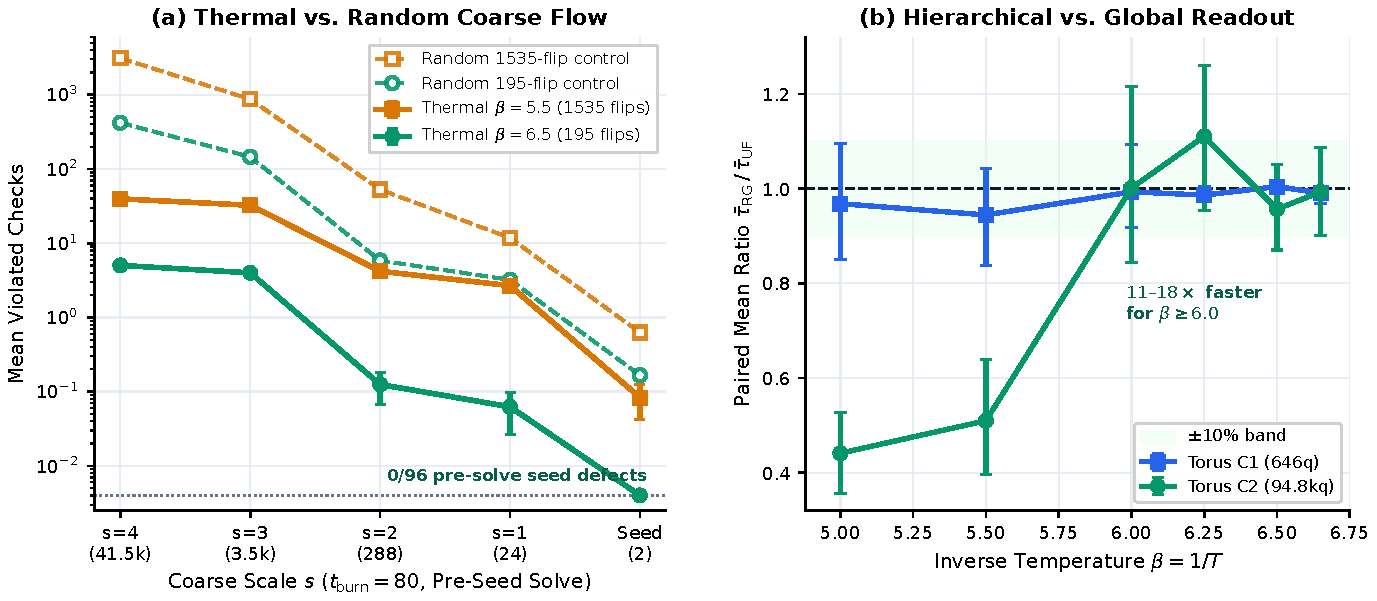
\includegraphics[width=0.98\textwidth]{../figures/fig_v19_4_readout.pdf}
  \caption{\textbf{Coarse Syndrome Confinement, Paired Readout, and Cadence Sensitivity.} \textbf{(a)}~Pre-seed-solve violated-check counts across scales $s = 4 \to 0$ on the $94{,}774$-qubit torus after burn-in $t_{\mathrm{burn}} = 80$ from $e(0) = 0$ ($96$ runs), comparing metastable thermal states (solid) against uniform random error configurations of the identical physical qubit weight (dashed). \textbf{(b)}~Paired cohort-mean lifetime ratio $\bar{\tau}_{\mathrm{RG}} / \bar{\tau}_{\mathrm{UF}}$ ($95\%$ bootstrap CI) between hierarchical cell readout and global Union-Find decoding on identical BKL trajectories. \textbf{(c)}~Paired detected failure times at $\beta = 6.5$ across checkpoint intervals $\eta \in [0, 0.50]$.}
  \label{fig:readout}
\end{figure*}

\subsection{Readout and Cadence Validation}

Proposition~\ref{prop:majority} motivates a fast hierarchical readout decoder (\texttt{rg\_dec}): starting at the finest scale, each $2 \times 2$ cell clears small local droplets, projects coarse syndromes one scale up via five-bit wall parity/majority rules until reaching the constant-size seed, lifts coarse corrections back down, and runs a final local cluster cleanup along lifted seam paths.

Before using coarse-graining as a confinement diagnostic, we define our state preparation operationally: evolving from $e(0) = 0$ for burn-in $t_{\mathrm{burn}} \in \{5, 20, 80, 320\} \ll \tau_X$ samples a \emph{metastable logical-sector state} rather than a globally mixed Gibbs state \cite{bergamaschi2025mixing}. Recording active coarse checks \emph{strictly before} any seed-level solve on $96$ independent $94{,}774$-qubit torus runs at $t_{\mathrm{burn}} = 80$ (and $t_{\mathrm{burn}} = 320$, where neutral $X$-stabilizer loops accumulate $\approx 908$ flipped qubits while active $Z$-checks remain steady at $5.4 \pm 0.3$; Fig.~\ref{fig:readout}a) shows $0/96$ nonzero pre-solve seed syndromes ($95\%$ one-sided Clopper--Pearson upper bound $3.07\%$) and $0/96$ decoded logical failures at $\beta = 6.5$. Passing uniform random errors of the exact same physical flip weight through the identical projection leaves $8/96$ ($t_{\mathrm{burn}} = 80$) and $25/96$ ($t_{\mathrm{burn}} = 320$) nonzero seed syndromes, isolating genuine thermal weld correlations from trivial check-count reduction.

Evaluating hierarchical readout and global Union-Find decoding on identical trajectories quantifies readout accuracy directly (Fig.~\ref{fig:readout}b; extended latencies in Appendix~\ref{app:wires}). Counting every readout checkpoint strictly prior to the first failure of either decoder, pre-failure logical classes agree on $99.99\text{--}100\%$ of cold checkpoints. On $646$-qubit Cycle~$1$ tori, paired cohort-mean ratios $\bar{\tau}_{\mathrm{RG}}/\bar{\tau}_{\mathrm{UF}}$ stay within $[0.986, 1.004]$ across $\beta \in [6.0, 6.65]$ (e.g., $1.004$, $95\%$ CI $[0.999, 1.014]$ at $\beta = 6.5$). On $94{,}774$-qubit Cycle~$2$ tori, hierarchical readout trails global decoding by $\approx 2\times$ in the warm regime ($\beta \le 5.5$) due to its lower single-shot threshold, whereas in the cold regime $\beta \in \{6.0, 6.25, 6.5, 6.65\}$ paired ratios are $1.001$ ($[0.84, 1.22]$), $1.110$ ($[0.95, 1.26]$), $0.957$ ($[0.87, 1.05]$), and $0.993$ ($[0.90, 1.09]$) while running $10.9\text{--}17.6\times$ faster ($1.03\,\mathrm{ms}$ vs.\ $16.2\,\mathrm{ms}$ at $\beta = 6.5$). Hard-capping the final lifted-seam cleanup at $64$ qubits (\texttt{rg\_strict}) fails prematurely on Cycle~$2$ ($\bar{\tau}_{\mathrm{strict}}/\bar{\tau}_{\mathrm{UF}} \approx 1.8 \times 10^{-3}$), confirming that \texttt{rg\_dec} is empirically fast on sparse thermal states rather than a worst-case bounded-radius decoder.

Paired readout-cadence audits at $\eta = 0, 0.05, 0.20$, and $0.50$ on Cycle~$1$ and at $\eta = 0.02, 0.05, 0.20$, and $0.50$ on Cycle~$2$ clarify checkpoint effects (Fig.~\ref{fig:readout}c). On $s = 0$ seeds, $\eta = 0.20$ and every-flip monitoring ($\eta = 0$) agree identically across all $2{,}000$ runs (and match exact $16$-state continuous-time Markov matrix inverses on $[[4,1,2]]$). On multi-cell codes, strict every-flip monitoring ($\eta = 0$) records brief boundary-crossing fluctuations that subsequently self-heal before the next $\eta = 0.05$ or $0.20$ checkpoint, making $\tau(\eta = 0.20)/\tau(\eta = 0)$ equal to $2.0\text{--}2.5$ on planar $C_1$ and $2.4\text{--}3.9$ on torus $C_1$. Between $\eta = 0.02$, $0.05$, and $0.20$, Cycle-$2$ lifetimes vary smoothly ($\tau(0.20)/\tau(0.02) = 1.46$, $95\%$ CI $[1.22, 1.81]$ on planar $C_2$ and $1.84$, $[1.32, 2.63]$ on torus $C_2$ at $\beta = 6.5$), and tightening readout fourfold to $\eta = 0.05$ preserves both the large planar cycle gain ($49.7\times$) and the torus cold gain ($3.28\times$).

\subsection{Spatial Packing and Routing Costs}

\begin{figure*}[t!]
  \centering
  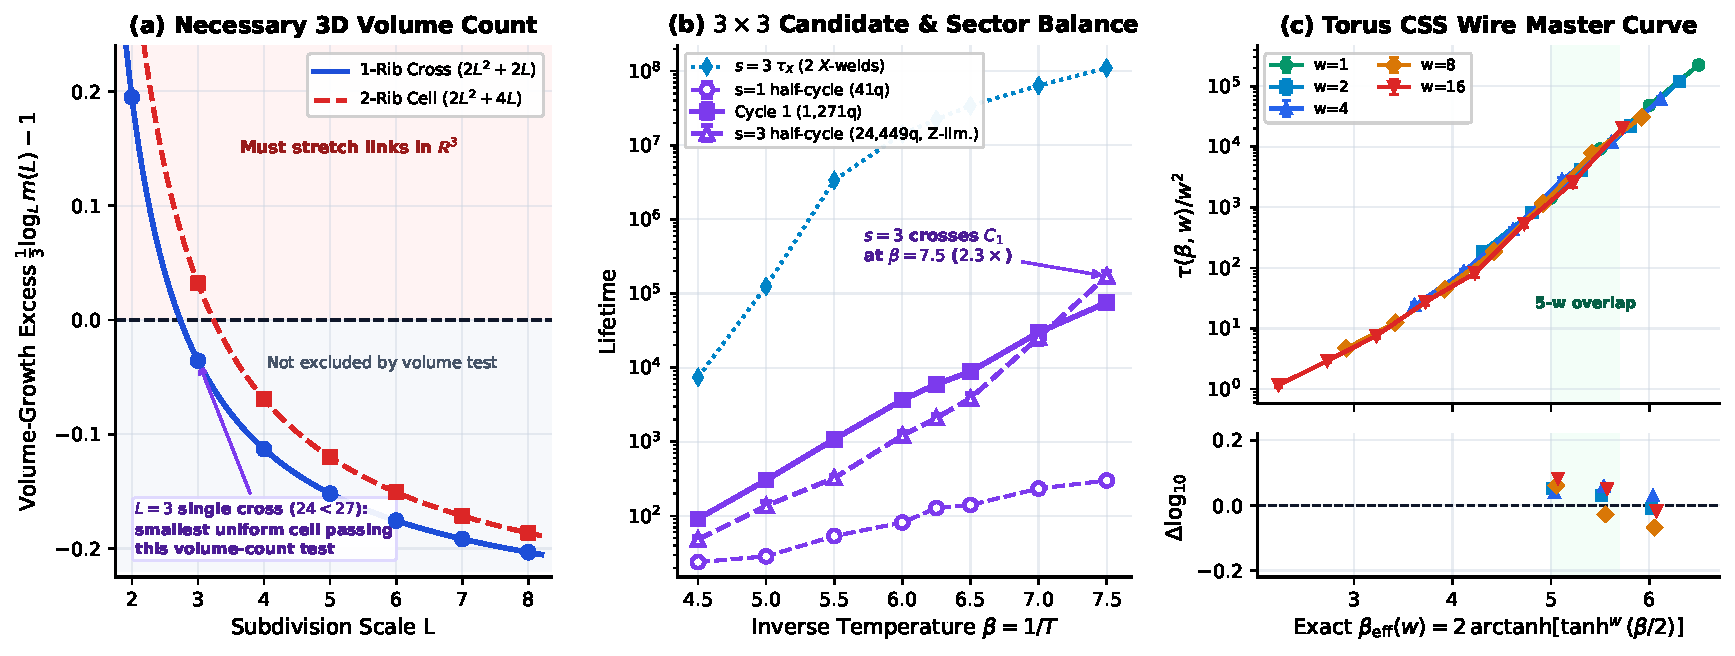
\includegraphics[width=0.98\textwidth]{../figures/fig_v19_5_implementation.pdf}
  \caption{\textbf{Spatial Volume Condition, $3 \times 3$ Sector Balance, and CSS Wire Dilution.} \textbf{(a)}~Volume-growth excess $\frac{1}{3}\log_L m(L) - 1$ for uniform $L \times L$ hierarchies in $\mathbb{R}^3$; positive values force link stretching, whereas $L = 3$ single-cross welding ($24 < 27$) is the smallest uniform member not excluded by this count. \textbf{(b)}~Planar $3 \times 3$ single-cross lifetimes up to $\beta = 7.5$: half-cycle $s = 3$ ($24{,}449$q) has $\tau_X > 10^8$ (blue diamonds) but is $Z$-limited below Cycle~$1$ ($1{,}271$q) until crossing above at $\beta = 7.5$ ($2.27 \pm 0.51\times$). \textbf{(c)}~Torus $X$-sector wire sweep ($N(w) = 646 + 288(w-1)$, $w \in \{1,2,4,8,16\}$) rescaled by $w^2$ against exact $\beta_{\mathrm{eff}}(w)$, shading the common five-curve support $\beta_{\mathrm{eff}} \in [5.0, 5.7]$ with matched-$\beta_{\mathrm{eff}}$ residuals below.}
  \label{fig:implementation}
\end{figure*}

Embedding our alternating physical interaction graph at bounded spatial density in $\mathbb{R}^3$ imposes a necessary ball-packing condition (Fig.~\ref{fig:implementation}a). In Appendix~\ref{app:packing}, we prove analytically for all steps $q \ge 1$ of a uniform $L \times L$ single-cross hierarchy that check-qubit incidence double counting enforces $N_q \ge \frac{3}{4}F_0\,m(L)^q$ with $m(L) = 2L^2 + 2L$, while physical Tanner-graph diameter satisfies the linear recurrence $D_q = O(L^q)$. Packing $N_q$ qubits inside a three-dimensional ball of radius $O(\ell_q D_q)$ forces maximum Euclidean link length $\ell_q = \Omega\bigl[(m(L)/L^3)^{q/3}\bigr]$. For $L = 2$ ($m(2) = 12 > 8$), links must stretch as $\ell_q = \Omega\bigl((3/2)^{q/3}\bigr) = \Omega(N_q^{0.0544})$. Within this uniform single-cross counting family, $2L^2 + 2L \le L^3$ first holds at integer $L = 3$ ($24 < 27$, whereas a two-rib $3 \times 3$ cell has $30 > 27$). Passing this necessary volume test neither constructs a collision-free $\mathbb{R}^3$ embedding nor rules out mixed schedules. Simulating the $3 \times 3$ single-cross planar hierarchy across $s = 1, 2, 3$ ($41 \to 1{,}271 \to 24{,}449$ qubits; Fig.~\ref{fig:implementation}b) highlights sector balance: at $s = 3$ (two $X$-welds, one $Z$-weld), $\tau_X$ exceeds $3.4 \times 10^7$ at $\beta = 6.5$, but sheet dilution lowers $\tau_Z$ below Cycle~$1$ across $\beta \le 7.0$ before $s = 3$ crosses above Cycle~$1$ at $\beta = 7.5$ ($G(7.5) = 2.27 \pm 0.51$).

Routing sheets and bridges into $\mathbb{Z}^3$ introduces distinct thermodynamic overheads depending on how interactions are realized. In BDL's $\ell = 8$ two-rib grid construction (\texttt{sq\_bdl\_8\_8\_r2}, $56{,}312$ qubits vs.\ $1{,}480$ qubits on the compact $L = 3$ two-rib direct graph, a $38.05\times$ qubit inflation while $1{,}480$q vs.\ $323$q is a $4.58\times$ direct-core change), there are zero weight-two wire checks; instead, $96.7\%$ of qubits sit at $Z$-degree two inside expanded two-dimensional surface-code collars where point defects wander across wider patches before meeting weld seams, reducing $\tau_Q(6.5)$ $440\times$ from $(1.74 \pm 0.19)\times 10^5$ to $394 \pm 33$ (Table~\ref{tab:lifetimes}).

A separate routing mechanism replaces long check legs by one-dimensional chains of $w$ weight-two ancilla checks, whose equilibrium Ising-wire physics was established by Qiu, Zoller, and Li \cite{qiu2020ising}. In Appendix~\ref{app:wires}, we specify an explicit CSS check-leg transformation on an $N_0$-qubit core with $M_Z$ $Z$-checks that introduces $M_Z(w - 1)$ ancillas ($N(w) = 646 + 288(w - 1)$ on torus $C_1$), preserves $H_X(w) H_Z(w)^T = 0$ and $K(w) = K(1)$, and yields an exact static marginal over core $X$-error syndromes $\sigma = H_Z(1)e_{\mathrm{core}}$.

\begin{proposition}[CSS Check-Leg Wire Marginal]
\label{prop:wires}
Under uniform $w$-link subdivision of one leg of each of the $M_Z$ $Z$-checks of $(H_X, H_Z)$, every allowed core $X$-syndrome $\sigma \in \operatorname{im} H_Z(1)$ has exact partition weight $Z(\sigma) = 2^{N_0 - \operatorname{rank} H_Z(1)} Z_0(\beta, w)^{M_Z} e^{-\beta_{\mathrm{eff}}(w)|\sigma|}$ with
\begin{equation}
  \beta_{\mathrm{eff}}(w) \;=\; 2\,\operatorname{arctanh}\!\Bigl[\bigl(\tanh(\beta / 2)\bigr)^w\Bigr],
  \label{eq:beta_eff}
\end{equation}
which satisfies $\beta_{\mathrm{eff}}(w) \approx \beta - \ln w$ only for $w e^{-\beta} \ll 1$ and $\beta_{\mathrm{eff}}(w) \to 0^+$ as $w \to \infty$ at fixed $\beta$.
\end{proposition}

Static marginal equivalence does not determine logical lifetime universally: at $\beta = 0$, wire endpoint spins flip at rate $1/2$ with total parity flip rate $1$ independent of $w$, violating any $w^2$ slowdown. In the cold, dilute, metastable regime ($w e^{-\beta} \ll 1$), however, single-defect diffusive crossing suggests the dynamical scaling model $\tau(\beta, w) \approx w^2 \tau_{\mathrm{core}}(\beta_{\mathrm{eff}}(w))$, under which $w = 1 \to 16$ on torus $C_1$ reduces $\tau_X(\beta = 6.5)$ $32\times$ ($2.24 \times 10^5 \to 7.04 \times 10^3$). Testing this dynamical model directly at exact matched $\beta_{\mathrm{eff}} \in \{5.0, 5.5, 6.0\}$ via $\beta(w) = 2\,\operatorname{arctanh}[\tanh(\beta_0/2)^{1/w}]$ gives fitted time exponents $\gamma = 2.06 \pm 0.05, 2.02 \pm 0.05$, and $1.97 \pm 0.05$ on the boundaryless $646$-qubit torus (RMS residual $0.034\text{--}0.054\text{ dex}$ against $w^2$ across the common five-curve support $\beta_{\mathrm{eff}} \in [5.0, 5.7]$; Fig.~\ref{fig:implementation}c), whereas open planar boundaries shift the kinetic exponent to $\gamma \approx 2.20\text{--}2.36$. This controlled $1$D wire sweep isolates ancilla-chain dilution on a fixed core and does not by itself predict the $2$D collar loss of the $\ell = 8$ grid.

\section{Discussion}

Simplifying BDL's Section~6.2 sheet-and-bridge hierarchy to compact $2 \times 2$ single-cross cells on bounded-degree graphs preserves two testable signatures of hierarchical thermal protection: local single-cell wall and majority contraction bounds, and large cold-regime lifetime gains ($55.9\times$ planar, $4.38\times$ torus at $\beta = 6.5$) across a completed alternating cycle at a $146.7\times$ qubit cost. At the same time, finite-size crossovers ($\beta \approx 6.1$ on tori) and un-welded half-cycle bottlenecks delimit where adding scale helps, while scale-selective coupling perturbations show that coarse Cycle-$1$ welds carry greater per-check thermal sensitivity than matched fine sub-cell welds even though both scales are required to sustain Cycle-$2$ protection.

Two scope limits frame future work. First, our evidence spans two nontrivial completed cycles under idealized single-qubit heat-bath dynamics on bounded-degree graphs; while programmable platforms can wire non-planar graphs \cite{guo2026neutral}, engineering passive stabilizer Hamiltonians and cold Markovian baths remains a distinct physical challenge, and a global multi-cell theorem for single-rib cells remains open. Second, in three-dimensional Euclidean space, uniform $2 \times 2$ cells must stretch links, leaving a constructive bounded-range $\mathbb{Z}^3$ embedding of the volume-compatible $3 \times 3$ cell---and its Cycle-$2$ completion---as concrete next steps.

\appendix

\section{Explicit CSS Rules and Local Proofs}
\label{app:css}

\emph{Seeds and sheaf CSS map.}---The planar seed $C_0$ (\texttt{seed\_planar\_11}, $[[2, 1, (2, 1)]]$) is a single square face with two opposite rough (\texttt{blue}) edges carrying qubits $q \in \{0, 1\}$ and two smooth (\texttt{red}, degree-$1$) edges carrying $d - 1 = 0$ qubits, giving $H_Z = (1\;1)$, $H_X$ empty ($0 \times 2$), $\bar{X} = X_0 X_1$ ($d_X = 2$), and $\bar{Z} = Z_0$ ($d_Z = 1$). The rotated torus seed (\texttt{seed\_rot\_torus\_422}, $[[4, 2, 2]]$) has $N = 4$ edges shared by two faces and two vertices, giving rank-$1$ matrices $H_X = H_Z = \bigl(\begin{smallmatrix}1&1&1&1\\1&1&1&1\end{smallmatrix}\bigr)$, $K = 4 - 1 - 1 = 2$, $\bar{X}_1 = X_0 X_1, \bar{X}_2 = X_0 X_2$, and $\bar{Z}_1 = Z_1 Z_3, \bar{Z}_2 = Z_2 Z_3$. At step $s$, subdividing edges by $L$, duplicating into copies $c \in \{0, 1\}$, and attaching bridge faces along interior rib grid lines assigns edge $e$ (with ordered incident faces $f_0 < \dots < f_{d-1}$) either one qubit coupled to all $f_j$ in $H_Z$ when $d = 2$ or $\mathrm{col}(e) = \mathrm{blue}$, or $d - 1$ qubits coupled to $\{f_j, f_{j+1}\}$ ($0 \le j \le d - 2$) when $\mathrm{col}(e) = \mathrm{red}$. At each vertex $v$ with incident faces $F_v$, local $X$-checks are minimal-weight basis vectors $\alpha \in \mathbb{F}_2^{F_v}$ satisfying $\alpha_{f_0} = \alpha_{f_j}$ on incident blue/$d=2$ edges and $\bigoplus_{j} \alpha_{f_j} = 0$ on incident red edges, mapped to qubits via $q(e)$ when $\alpha_{f_0} = 1$ (blue/$d=2$) and $q_j(e)$ when $\bigoplus_{l \le j} \alpha_{f_l} = 1$ (red). Every $X$-row shares even overlap ($0$ or $2$) with every $Z$-face row, establishing $H_X H_Z^T = 0 \pmod 2$.

\emph{Proof of Proposition~\ref{prop:majority}.}---Complement all $12$ bits if needed so $r = \sum_{i=0}^3 c_i \le 2$. Always $C \le 2$, so $V \ge 5$ suffices whenever $C = 2$, and $V \ge 3$ suffices when $C = 1$. If $r = 2$, each sheet has at least two violated triples and $\chi(c_0,c_1,c_2,c_3) = 1$, giving $V \ge 5$. If $r = 1$ and $V \le 4$, at least one sheet violates at most one triple and must therefore be all zero; hence $n_i \ge 3$ can hold only on the unique wall with $c_i = 1$, giving $C \le 1$, and if $n_i \ge 3$ there, the other sheet has $b_i = b_{i+1} = 1$, forcing at least two violations on that sheet plus one on the zero sheet and one at the center ($V \ge 4 \implies C/V \le 1/4 < 2/5$). If $r = 0$ and $V \le 4$, either one sheet is all zero or each sheet has at most one $1$; in both cases $n_i \le 2$ on every wall, so $C = 0$.

\emph{Physical parity basis and coarse inversion.}---In our CSS code, an interior $2 \times 2$ even-weld cell has $19$ interior parity qubits: eight three-face \texttt{red} rib seams ($2$ qubits each, contributing $(a_i \oplus a_{i+1}) + (a_{i+1} \oplus c_i)$ on Sheet~$0$ and $(b_i \oplus b_{i+1}) + (b_{i+1} \oplus c_i)$ on Sheet~$1$) plus one four-face central vertical \texttt{red} edge ($3$ qubits, contributing $(c_0 \oplus c_1) + (c_1 \oplus c_2) + (c_2 \oplus c_3)$). Each violated triple contributes $1$ or $2$ parity violations and the center contributes $1$ to $3$; $3$ central violations require alternating $c = 0101$ or $1010$, which forces $\ge 2$ violated triples per sheet and $V \ge 5$, so $V \le V_{\mathrm{phys}} \le 2V + 1 \le \frac{11}{5}V$ (tight at $a = b = 0000, c = 0101$). Lifting a coarse face assignment $y \in \mathbb{F}_2^{F_{\mathrm{coarse}}}$ by setting all $12$ subfaces of cell $P$ to $y_P$ sets $(H_Z^{\mathrm{fine}})^T(\pi^* y) = 0$ on all interior qubits and sets all five qubits of each shared wall $(P, P')$ to $y_P \oplus y_{P'} = [(H_Z^{\mathrm{coarse}})^T y]_{(P, P')}$, making simultaneous four-wall inversion globally consistent across neighboring cells.

\section{Physical Graph Count and Diameter Bounds}
\label{app:packing}

For any uniform $L \times L$ ($L \ge 2$) single-cross hierarchy, each step subdivides every face into $L^2$ subfaces across two copies ($2L^2$) and adds $2L$ bridge faces along the two interior cross lines, so $F_q = F_0 m(L)^q$ with $m(L) = 2L^2 + 2L$. For $q \ge 1$, every face $Z$-check has weight $\ge 3$ (at most one side of a boundary square can be a degree-$1$ smooth edge), while by construction every physical qubit belongs to $2$ faces (for $d = 2$ or red seams) or $d \le 4$ faces (for blue seams). Double-counting $Z$-check--qubit incidences $I_q$ gives $3 F_q \le I_q \le 4 N_q$, hence $N_q \ge \frac{3}{4}F_0 m(L)^q$ for all $q \ge 1$.

Let $\Delta_q$ be the vertex diameter of the 2-complex $C_q$. Under step $q \to q + 1$, every parent edge becomes a path of $\le L$ subedges, every subdivided face plus bridge has internal vertex diameter $\le 2L + 2$, and the two copies meet at distance $1$ along every rib vertex, giving $\Delta_{q+1} \le L\Delta_q + (2L + 3)$. Dividing by $L^{q+1}$ and summing the geometric series yields $\Delta_q \le L^q\bigl[\Delta_0 + (2L + 3)/(L - 1)\bigr] = O(L^q)$. Because every non-smooth edge carries at least one physical qubit and adjacent faces on a degree-$d \le 4$ seam are linked by a chain of $\le 3$ qubits, physical Tanner-graph qubit diameter satisfies $D_q \le 3\Delta_q + 2 = O(L^q)$. If qubits embed in $\mathbb{R}^3$ at bounded spatial density with maximum link length $\ell_q$, all $N_q$ qubits lie within Euclidean radius $\ell_q D_q$, so $\frac{3}{4}F_0 m(L)^q \le N_q \le C(1 + \ell_q D_q)^3$, giving $\ell_q = \Omega\bigl[(m(L)/L^3)^{q/3}\bigr]$.

\section{CSS Wire Reduction and Decoder Timings}
\label{app:wires}

\emph{Proof of Proposition~\ref{prop:wires}.}---Given core $(H_X^{(1)}, H_Z^{(1)})$ on $N_0$ qubits with $M_Z$ $Z$-checks $r_c = \{q_c\} \sqcup R_c$, add $M_Z(w - 1)$ wire qubits $u_{c,1},\dots,u_{c,w-1}$ ($N(w) = N_0 + M_Z(w - 1)$). Replace $r_c$ in $H_Z(w)$ by $r_{c,1} = R_c \sqcup \{u_{c,1}\}$, $r_{c,k} = \{u_{c,k-1}, u_{c,k}\}$ ($2 \le k \le w - 1$), and $r_{c,w} = \{u_{c,w-1}, q_c\}$; append $\{u_{c,1},\dots,u_{c,w-1}\}$ to every row of $H_X$ and $\bar{X}$ containing $q_c$. Each extended $X$-row meets $r_{c,1}$ in $|s \cap r_c| \equiv 0 \pmod 2$ qubits and meets $r_{c,2\dots w}$ in $0$ or $2$ qubits, so $H_X(w)H_Z(w)^T = 0$. Since $\bigoplus_{k=1}^w r_{c,k} = r_c$ while $r_{c,2\dots w}$ have distinct private pivots $u_{c,k-1}$, $\operatorname{rank} H_Z(w) = \operatorname{rank} H_Z(1) + M_Z(w - 1)$ and $\operatorname{rank} H_X(w) = \operatorname{rank} H_X(1)$, preserving $K(w) = K(1)$ (certified on $646 + 288(w - 1)$ torus codes where $\operatorname{rank} H_Z(1) = 285, \operatorname{rank} H_X(1) = 359, K = 2$). For any fixed $e_{\mathrm{core}} \in \mathbb{F}_2^{N_0}$ with $\sigma = H_Z(1)e_{\mathrm{core}}$, varying $u_c \in \{0,1\}^{w-1}$ bijects onto bond defects $(\tau_{c,2},\dots,\tau_{c,w}) \in \{0,1\}^{w-1}$ with $\tau_{c,1} = \sigma_c \oplus \bigoplus_{k=2}^w \tau_{c,k}$, giving $\sum_{u_c} e^{-\beta\sum_{k=1}^w \tau_{c,k}} = \frac{1}{2}[(1+e^{-\beta})^w + (-1)^{\sigma_c}(1-e^{-\beta})^w] = Z_0 e^{-\beta_{\mathrm{eff}}(w)\sigma_c}$. Summing over the $|\ker H_Z(1)| = 2^{N_0 - \operatorname{rank} H_Z(1)}$ core states in the fiber of $\sigma$ yields Proposition~\ref{prop:wires}.

\emph{Decoder runtime benchmark.}---Per-call single-core decode latencies on thermal BKL checkpoints (x86-64 SubMIT cluster nodes, \texttt{g++ -O3}) are $0.033\,\mathrm{ms}$ (\texttt{uf}) vs.\ $0.011\,\mathrm{ms}$ (\texttt{rg\_dec}, $3.0\times$) on the $646$-qubit Cycle-$1$ torus ($\beta = 6.5$), $16.2\,\mathrm{ms}$ vs.\ $1.03\,\mathrm{ms}$ ($15.8\times$) on the $94{,}774$-qubit Cycle-$2$ torus at $\beta = 6.5$ ($9.06\,\mathrm{ms}$ vs.\ $0.83\,\mathrm{ms}$, $10.9\times$ at $\beta = 6.65$; $28.3\,\mathrm{ms}$ vs.\ $1.77\,\mathrm{ms}$, $16.0\times$ at $\beta = 6.0$), and $295\,\mathrm{ms}$ vs.\ $64.5\,\mathrm{ms}$ ($4.6\times$) across the single-sector $2 \times 2$ planar series at $N = 322{,}159$ ($\beta = 2.20$).

\bibliographystyle{apsrev4-2}
\bibliography{references}

\end{document}
